\renewcommand{\thesubsection}{\textcolor{red}{\Roman{section}.\arabic{subsection}}}
\renewcommand{\thesubsubsection}{\textcolor{red}{\Roman{section}.\arabic{subsection}.\alph{subsubsection}}}

\setcounter{section}{0}
\sndEnTeteCoursTrois

\begin{mdframed}[style=titr, leftmargin=60pt, rightmargin=60pt, innertopmargin=7pt, innerbottommargin=7pt, innerrightmargin=8pt, innerleftmargin=8pt]

\begin{center}
\large{\textbf{Chapitre 3 : \'{E}mission, propagation et perception du son}}
\end{center}
\end{mdframed}
Dans ce chapitre, nous allons nous intéresser aux propriétés du son : comment émettre un signal sonore ? Comment se propage-t'il ? \`{A} quelle vitesse ? Comment modéliser un signal sonore pour décrire des sons de la vie de tous les jours ?

\begin{tcolorbox}[colback=blue!5!white,colframe=blue!75!black,title=Mots clés du chapitre :]
Emission, propagation, vitesse du son dans l'air, signal périodique, fréquences audibles, hauteur, timbre, niveau d'intensité sonore.
\end{tcolorbox}


\section{\'{E}mission et propagation d'un signal sonore}
\subsection{Approche expérimentale de l'émission}

\textcolor{green}{\underline{Expérience 1 :}} On place une bougie allumée devant la membrane d'un haut-parleur (ici une enceinte branchée à un smartphone). On met une musique sur le smartphone qui est émise par le haut-parleur.\\
\textbf{Observations :} \gap{..................................................................}\\
\gap{........................................................................................................................................}\\
\gap{........................................................................................................................................}\\
\gap{........................................................................................................................................}\\
\gap{................................................................................................}\\
\begin{wrapfigure}{r}{0.3\textwidth}
\vspace{-7cm}
    \centering
     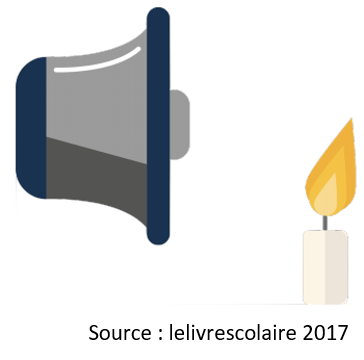
\includegraphics[width=0.32\textwidth]{Images/Chapitre_3/Haut_parleur_bougie.PNG}
   \end{wrapfigure}

\begin{tcolorbox}[colback=red!5!white,colframe=red!75!black,title=\textbf{Propriété de l'émission d'un son : }]
L'émission d'un signal sonore par un objet appelé \textcolor{red}{émetteur} résulte de la vibration de cet objet. Cette vibration se transmet fait vibrer les molécules dans l'air de proche en proche pour permettre sa \textcolor{red}{propagation}.
\end{tcolorbox}

\textcolor{blue}{Vidéo : les insectes les plus bruyants du monde !} \url{https://www.youtube.com/watch?v=qveMTTSAQPQ}
\begin{tcolorbox}[colback=red!5!white,colframe=red!75!black,title=\textbf{Caisse de résonance : }]
Une \textcolor{red}{caisse de résonance}permet de sélectionner et d'amplifier, c'est-à-dire augmenter son \textcolor{red}{amplitude} certains sons.
\end{tcolorbox}

\textbf{\underline{Exemple de caisse de résonance :}} Les instuments de musiques : flûte, guitare acoustique, contrebasse, etc.


\subsection{Approche expérimentale de la propagation}
\textcolor{green}{\underline{Expérience 2 :}} On place un réveil ou une alarme sur le plateau d'une cloche à vide. On met l'alarme en marche et on fait progressivement le vide (on retire l'air) sous la cloche. On mesure l'intensité du son au cours de l'expérience grâce à un sonomètre.
\begin{center}
    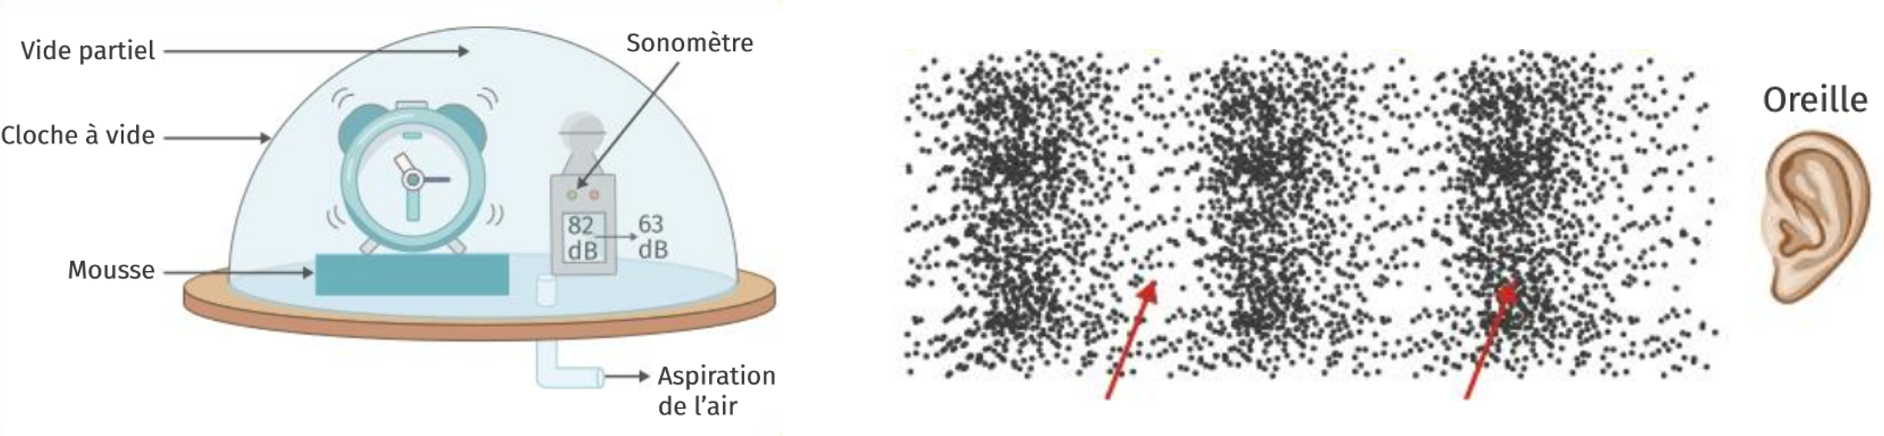
\includegraphics[scale=0.57]{Images/Chapitre_3/Propagation_exp.png}
\end{center}

\textbf{Observations :} \gap{...............................................................................................................}\\
\gap{.......................................................................................................................................}\\
\gap{.......................................................................................................................................}\\
\gap{.......................................................................................................................................}\\

\begin{tcolorbox}[colback=red!5!white,colframe=red!75!black,title=\textbf{Propriété de la propagation du son : }]
Le son a besoin d'un \textcolor{red}{milieu matériel} pour se propager. Le signal se propage par suite de compressions et dilatations du milieu de propagation.
\end{tcolorbox}

Pour revoir l'expérience de la cloche à vide en vidéo : \url{https://www.youtube.com/watch?v=BC9Pod4cnpk}

\importantbox{Un signal sonore peut se propager dans un autre milieu matériel que l'air. Les baleines à bosses chantent sous l'eau pour communiquer entre elles et même choisir leur partenaire de reproduction sur des milliers de kilomètres ! C'est possible car dans l'eau, le son se propage à 500~m.s$^{-1}$, qu'en-est-il dans l'air ?}

\begin{Large}
    \ding{45}
\end{Large}\textbf{Exercice DOC : l'alcool dénaturé.}


\section{Vitesse de propagation d'un signal sonore}
\begin{Large}
    \ding{43}
\end{Large}
Voir TP 7 : Mesure de la vitesse du son dans l'air.
\subsection{Définition}
\begin{tcolorbox}[colback=green!5!white,colframe=green!75!black,title=\textbf{Vitesse de propagation :}]
La \textcolor{red}{vitesse de propagation} $v$ d'un signal sonore est définie comme le rapport de la distance $d$ parcourue par ce signal sur le temps (ou durée) de propagation $\Delta t$ associé :
\begin{empheq}[box=\fbox]{equation*}
    v = \frac{d}{\Delta t}
\end{empheq}
$v$ s'exprime en m.s$^{-1}$, $d$ en m et $\Delta t$ en s.
\end{tcolorbox}
\subsection{Influence du milieu et de ses caractéristiques sur la vitesse de propagation du son}
\subsubsection{La température}
\`{A} partir du document 2 dans le TP 7 : \textit{Mesure de la vitesse des ondes sonores dans l'air}, compléter le tableau suivant :
\begin{center}
    \begin{tabular}{|C{0.4}|C{0.09}|C{0.09}|C{0.09}|C{0.09}|C{0.09}|}
\hline
     Température (en $\degreCelsius$) & -10 & 0 & 10 & 20 & 30 \\
     \hline 
     Vitesse de propagation du son dans l'air (en m.s$^{-1}$) & 325 & 332 & 337 & 343 & 349 \\
     \hline
\end{tabular}
\end{center}
\subsubsection{Le milieu de propagation}
\begin{center}
    \begin{tabular}{|C{0.4}|C{0.09}|C{0.09}|C{0.09}|C{0.09}|C{0.09}|}
\hline
     Milieu & air & eau & béton & acier \\
     \hline 
     Vitesse de propagation du son dans le milieu à 15$\degreCelsius$ (en m.s$^{-1}$) & 340 & 1480 & 3100 & 5600 \\
     \hline
\end{tabular}
\end{center}

\begin{tcolorbox}[colback=red!5!white,colframe=red!75!black,title=\textbf{Bilan sur la propagation du son dans un milieu : }]
La vitesse de propagation du son dépend du \textcolor{red}{milieu matériel de propagation} et des \textcolor{red}{caractéristiques physiques} de ce milieu (température, masse volumique, compressibilité) de celui-ci.\\

On retiendra qu'à T=15$\degreCelsius$ : 
\begin{empheq}[box=\fbox]{equation*}
    v_{son, air} \simeq 340~\text{m.s$^{-1}$}
\end{empheq}

\end{tcolorbox}


\subsection{Comparaison de $v_{son, air}$ avec d'autres valeurs de vitesses}
Pour bien se rendre compte de la rapidité relative du son dans l'air, voici un tableau avec d'autres valeurs de vitesses couramment rencontrées :
\begin{center}
    \begin{tabular}{|c|c|c|c|c|c|c|c|}
\hline
     Exemple & Escargot & Usain Bolt & Guépard & Son (à 15$\degreCelsius$)  & Ariane 5 & Lumière \\
     \hline 
     Vitesse (en m/s) & 0,001 & 10,44 & 36,1 & 340 & 10410 & $300 000 000$\\
     \hline
\end{tabular}
\end{center}

\begin{wrapfigure}{r}{0.38\textwidth}
\vspace{-0.6cm}
    \centering
     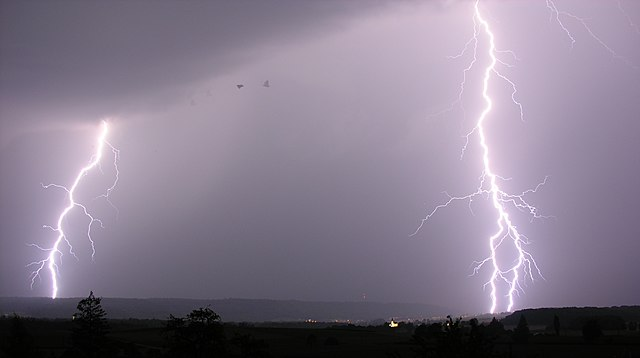
\includegraphics[width=0.38\textwidth]{Images/Chapitre_3/Eclair.JPG}
   \end{wrapfigure}
\begin{mdframed}[style=autreexo]
\textbf{\bsc{Exercice de cours 1} - Distance d'un orage}\\
Un observateur observe un orage. Soudain, il voit le ciel s'éclairer et un éclair tomber. Il déclanche alors un chronomètre et mesure $\Delta t = 2,07$~s au moment où le grondement du tonnerre lui parvient. \`{A} quelle distance de l'observateur se situe l'éclair qui vient de tomber ?
\end{mdframed}
\textit{Réponse : } \gap{.......................................................................................................................}\\
\gap{.......................................................................................................................................}\\
\gap{.......................................................................................................................................}\\
\gap{.......................................................................................................................................}
\section{Les signaux sonores périodiques}
Nous nous intéressons dans cette section à décrire les caractéristiques d'un signal sonore : quels outils mathématiques peut-on utiliser pour décrire un son plus ou moins fort ? plus ou moins aigu ? Comment peut-on visualiser un signal sonore en physique ?
\subsection{\og Voir \fg un son à l'aide d'une chaîne de mesure}
\begin{tcolorbox}[colback=green!5!white,colframe=green!75!black,title=\textbf{Microphone et enregistrement:}]
Un microphone est un capteur qui convertit un signal sonore reçu en une tension électrique $U$ en volt. Le signal électrique produit par le microphone est ensuite enregistré sur une carte de mesure relié à un ordinateur qui permet d'afficher et anayser le signal sonore.
\begin{center}
    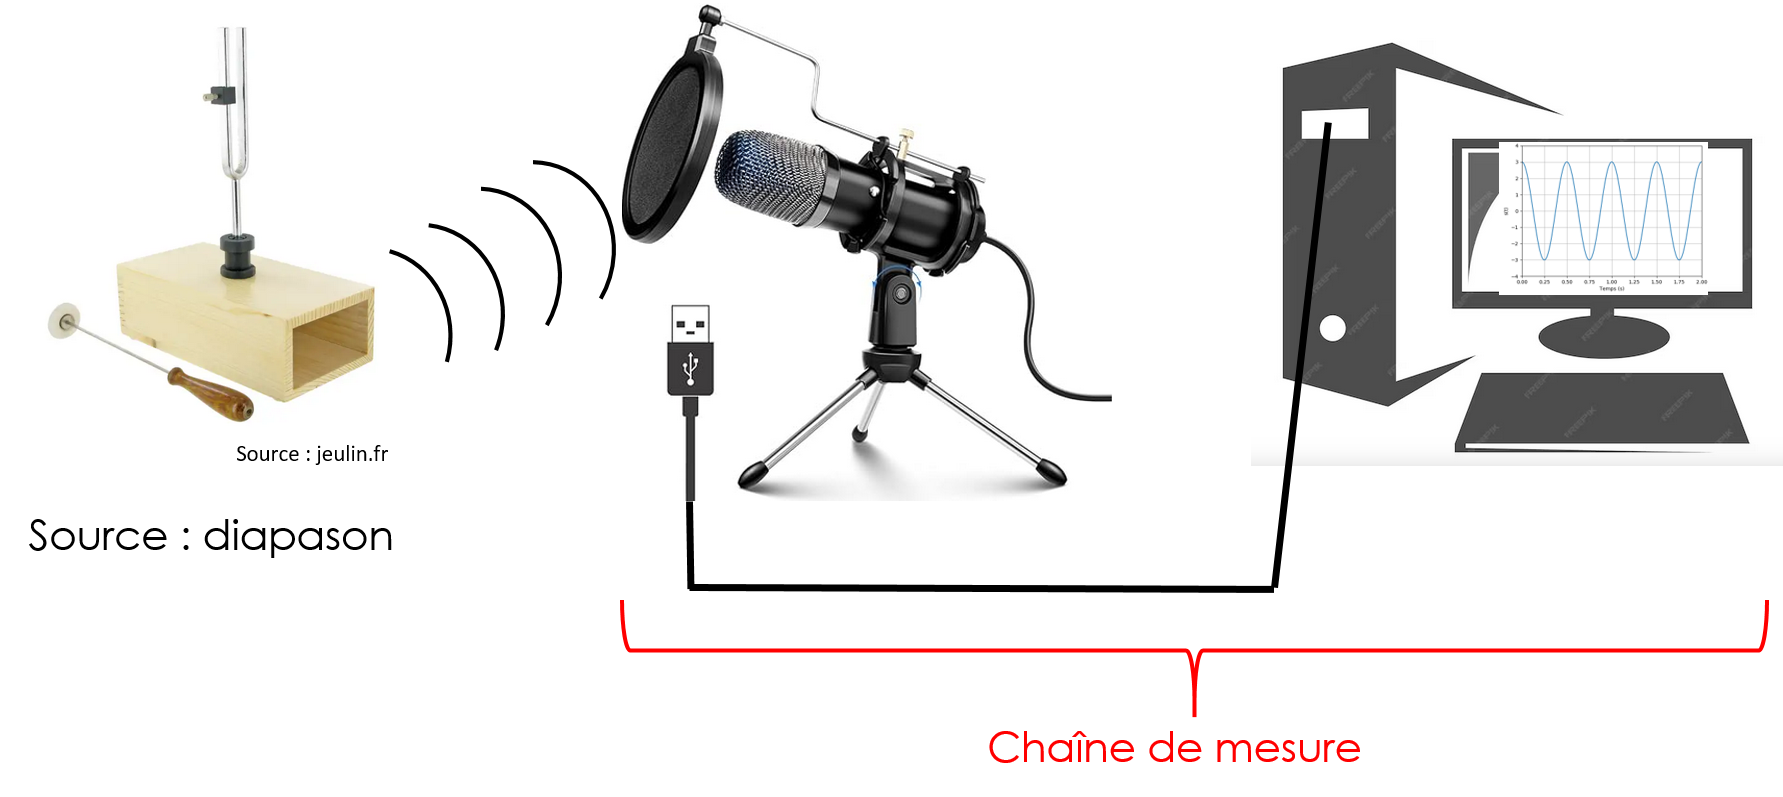
\includegraphics[scale = 0.5]{Images/Chapitre_3/Chaine_mesure.png}
\end{center}
\end{tcolorbox}
\subsection{Définition d'un signal sonore périodique}
\textcolor{green}{Expérience 3 :} On joue une note à l'aide d'un diapason (voir la figure ci-dessus), le signal est amplifié par une caisse de résonance devant laquelle est placé un microphone. Le signal produit est le suivant :
\begin{center}
    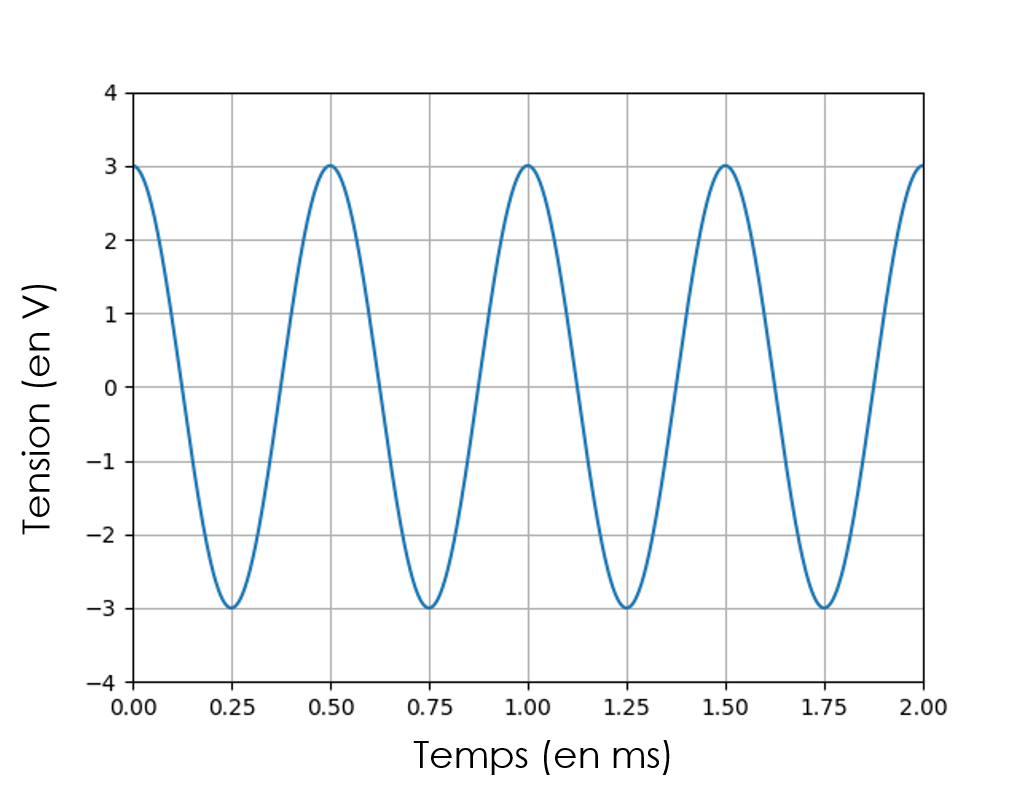
\includegraphics[scale=0.5]{Images/Chapitre_3/Signal_diapason.PNG}
\end{center}
\begin{tcolorbox}
[colback=green!5!white,colframe=green!75!black,title=\textbf{Signal périodique :}]
Un signal sonore \textcolor{red}{périodique} est un signal qui se \textcolor{red}{reproduit à l'identique} au cours du temps. 
\end{tcolorbox}

\section{Perception d'un son}